% Generated from the fixed rq3-cells.csv and checked against its outcome macros.
\begin{figure}[!htbp]
\centering
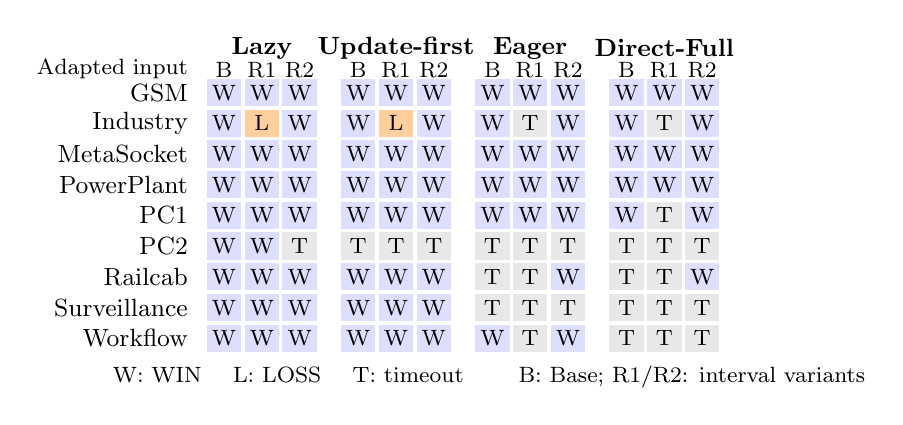
\begin{tikzpicture}[x=.48cm,y=.39cm,font=\small,
    cell/.style={draw=white,minimum width=4.5mm,minimum height=3.6mm,inner sep=0pt,font=\footnotesize},
    win/.style={cell,fill=blue!13,text=black},
    loss/.style={cell,fill=orange!38,text=black},
    timeout/.style={cell,fill=black!9,text=black}]
\node[anchor=east,font=\footnotesize] at (-.7,.75) {Adapted input};
\node[font=\small\bfseries] at (1.00,1.45) {Lazy};
\node[font=\footnotesize] at (0.00,.75) {B};
\node[font=\footnotesize] at (1.00,.75) {R1};
\node[font=\footnotesize] at (2.00,.75) {R2};
\node[win] at (0.00,0.00) {W};
\node[win] at (1.00,0.00) {W};
\node[win] at (2.00,0.00) {W};
\node[win] at (0.00,-1.00) {W};
\node[loss] at (1.00,-1.00) {L};
\node[win] at (2.00,-1.00) {W};
\node[win] at (0.00,-2.00) {W};
\node[win] at (1.00,-2.00) {W};
\node[win] at (2.00,-2.00) {W};
\node[win] at (0.00,-3.00) {W};
\node[win] at (1.00,-3.00) {W};
\node[win] at (2.00,-3.00) {W};
\node[win] at (0.00,-4.00) {W};
\node[win] at (1.00,-4.00) {W};
\node[win] at (2.00,-4.00) {W};
\node[win] at (0.00,-5.00) {W};
\node[win] at (1.00,-5.00) {W};
\node[timeout] at (2.00,-5.00) {T};
\node[win] at (0.00,-6.00) {W};
\node[win] at (1.00,-6.00) {W};
\node[win] at (2.00,-6.00) {W};
\node[win] at (0.00,-7.00) {W};
\node[win] at (1.00,-7.00) {W};
\node[win] at (2.00,-7.00) {W};
\node[win] at (0.00,-8.00) {W};
\node[win] at (1.00,-8.00) {W};
\node[win] at (2.00,-8.00) {W};
\node[font=\small\bfseries] at (4.55,1.45) {Update-first};
\node[font=\footnotesize] at (3.55,.75) {B};
\node[font=\footnotesize] at (4.55,.75) {R1};
\node[font=\footnotesize] at (5.55,.75) {R2};
\node[win] at (3.55,0.00) {W};
\node[win] at (4.55,0.00) {W};
\node[win] at (5.55,0.00) {W};
\node[win] at (3.55,-1.00) {W};
\node[loss] at (4.55,-1.00) {L};
\node[win] at (5.55,-1.00) {W};
\node[win] at (3.55,-2.00) {W};
\node[win] at (4.55,-2.00) {W};
\node[win] at (5.55,-2.00) {W};
\node[win] at (3.55,-3.00) {W};
\node[win] at (4.55,-3.00) {W};
\node[win] at (5.55,-3.00) {W};
\node[win] at (3.55,-4.00) {W};
\node[win] at (4.55,-4.00) {W};
\node[win] at (5.55,-4.00) {W};
\node[timeout] at (3.55,-5.00) {T};
\node[timeout] at (4.55,-5.00) {T};
\node[timeout] at (5.55,-5.00) {T};
\node[win] at (3.55,-6.00) {W};
\node[win] at (4.55,-6.00) {W};
\node[win] at (5.55,-6.00) {W};
\node[win] at (3.55,-7.00) {W};
\node[win] at (4.55,-7.00) {W};
\node[win] at (5.55,-7.00) {W};
\node[win] at (3.55,-8.00) {W};
\node[win] at (4.55,-8.00) {W};
\node[win] at (5.55,-8.00) {W};
\node[font=\small\bfseries] at (8.10,1.45) {Eager};
\node[font=\footnotesize] at (7.10,.75) {B};
\node[font=\footnotesize] at (8.10,.75) {R1};
\node[font=\footnotesize] at (9.10,.75) {R2};
\node[win] at (7.10,0.00) {W};
\node[win] at (8.10,0.00) {W};
\node[win] at (9.10,0.00) {W};
\node[win] at (7.10,-1.00) {W};
\node[timeout] at (8.10,-1.00) {T};
\node[win] at (9.10,-1.00) {W};
\node[win] at (7.10,-2.00) {W};
\node[win] at (8.10,-2.00) {W};
\node[win] at (9.10,-2.00) {W};
\node[win] at (7.10,-3.00) {W};
\node[win] at (8.10,-3.00) {W};
\node[win] at (9.10,-3.00) {W};
\node[win] at (7.10,-4.00) {W};
\node[win] at (8.10,-4.00) {W};
\node[win] at (9.10,-4.00) {W};
\node[timeout] at (7.10,-5.00) {T};
\node[timeout] at (8.10,-5.00) {T};
\node[timeout] at (9.10,-5.00) {T};
\node[timeout] at (7.10,-6.00) {T};
\node[timeout] at (8.10,-6.00) {T};
\node[win] at (9.10,-6.00) {W};
\node[timeout] at (7.10,-7.00) {T};
\node[timeout] at (8.10,-7.00) {T};
\node[timeout] at (9.10,-7.00) {T};
\node[win] at (7.10,-8.00) {W};
\node[timeout] at (8.10,-8.00) {T};
\node[win] at (9.10,-8.00) {W};
\node[font=\small\bfseries] at (11.65,1.45) {Direct-Full};
\node[font=\footnotesize] at (10.65,.75) {B};
\node[font=\footnotesize] at (11.65,.75) {R1};
\node[font=\footnotesize] at (12.65,.75) {R2};
\node[win] at (10.65,0.00) {W};
\node[win] at (11.65,0.00) {W};
\node[win] at (12.65,0.00) {W};
\node[win] at (10.65,-1.00) {W};
\node[timeout] at (11.65,-1.00) {T};
\node[win] at (12.65,-1.00) {W};
\node[win] at (10.65,-2.00) {W};
\node[win] at (11.65,-2.00) {W};
\node[win] at (12.65,-2.00) {W};
\node[win] at (10.65,-3.00) {W};
\node[win] at (11.65,-3.00) {W};
\node[win] at (12.65,-3.00) {W};
\node[win] at (10.65,-4.00) {W};
\node[timeout] at (11.65,-4.00) {T};
\node[win] at (12.65,-4.00) {W};
\node[timeout] at (10.65,-5.00) {T};
\node[timeout] at (11.65,-5.00) {T};
\node[timeout] at (12.65,-5.00) {T};
\node[timeout] at (10.65,-6.00) {T};
\node[timeout] at (11.65,-6.00) {T};
\node[win] at (12.65,-6.00) {W};
\node[timeout] at (10.65,-7.00) {T};
\node[timeout] at (11.65,-7.00) {T};
\node[timeout] at (12.65,-7.00) {T};
\node[timeout] at (10.65,-8.00) {T};
\node[timeout] at (11.65,-8.00) {T};
\node[timeout] at (12.65,-8.00) {T};
\node[anchor=east] at (-.7,0.00) {GSM};
\node[anchor=east] at (-.7,-1.00) {Industry};
\node[anchor=east] at (-.7,-2.00) {MetaSocket};
\node[anchor=east] at (-.7,-3.00) {PowerPlant};
\node[anchor=east] at (-.7,-4.00) {PC1};
\node[anchor=east] at (-.7,-5.00) {PC2};
\node[anchor=east] at (-.7,-6.00) {Railcab};
\node[anchor=east] at (-.7,-7.00) {Surveillance};
\node[anchor=east] at (-.7,-8.00) {Workflow};
\node[anchor=west,font=\footnotesize] at (-3.2,-9.25)
  {W: WIN \quad L: LOSS \quad T: timeout \qquad B: Base; R1/R2: interval variants};
\end{tikzpicture}
\caption{Every fixed-budget contract--method outcome. Each tile is one of the same
\ApplicationModels{} inputs $\times$ three requirement variants, under a
1,200~s cap and 64~GiB heap. WIN and LOSS are completed decisions; timeout leaves
feasibility unresolved. The methods change exploration, keeping entries,
successors and goals fixed. The comparison evaluates complete exploration procedures.
Workflow/R2's Direct-Full tile uses the recorded same-setting timeout after
interruption; both attempts are retained.}
\label{fig:rq3-outcomes}
\Description{A grid of all 27 contracts for each of four methods. Lazy has 25 WIN,
one LOSS at Industry R1 and one timeout at PC2 R2. Update-first has 23 WIN, one LOSS
and three timeouts. Eager has 17 WIN and ten timeouts. Direct-Full has 14 WIN and
13 timeouts. Every completed paired decision agrees.}
\end{figure}
